% Copyright 2023 Kieran W Harvie. All rights reserved.

\chapter{Automatic Differentiation}
Automatic Differentiation is a collection of techniques for algorithmically calculating the partial derivative of a function in some general way.
The core observation is that if the functions can be expressed in terms of elementary functions with known partial derivatives we should be able to use the chain rule to calculate the partial derivative of the original function.
General

\section{A Tale of Two Derivative}
Partial and total.
Chain rule.
$\nabla$ operator maybe an appendix for vectors?
\[\frac{d\,f}{d\,t} = \sum_i \frac{\partial f}{\partial x_i}\frac{d\,x_i}{d\,t} = \nabla f \cdot \left(\frac{d\,x_0}{d\,t},\frac{d\,x_1}{d\,t},\frac{d\,x_2}{d\,t},\dots\right)\]

\section{Forward Accumulation}
\subsection{Dual Numbers}
Like how we get Complex numbers from Real numbers by adjoining a new number $i$ such that $i^2=-1$ we get the Dual numbers by adjoining a new number $\epsilon$, 
called the infinitesimal, 
such that $\epsilon^2 = 0$.

Some properties aren't that special:
\[(x+x'\epsilon) + (y+y'\epsilon) = (x+y)+(x'+y')\epsilon\]

But consider what happens for multiplication and division:
\begin{equation*}
\begin{aligned}
(x+x'\epsilon)(y+y'\epsilon) =& xy+(x'y+xy')\epsilon+x'y'\epsilon^2 \\
=& xy+(x'y+xy')\epsilon \\
\frac{x+x'\epsilon}{y+y'\epsilon} =& \frac{(x+x'\epsilon)(y-y'\epsilon)}{(y+y'\epsilon)(y-y'\epsilon)} \\
 =& \frac{xy+(x'y-xy')\epsilon-x'y'\epsilon^2}{y^2-y'^2\epsilon^2} \\
 =& \frac{x}{y}+\frac{x'y-xy'}{y^2}\epsilon \\
\end{aligned}
\end{equation*}

Define:
$f\left(\dual{u}{u'},\dual{v}{v'}\right) = \dual{f(u,v)}{\nabla f(u,v) \cdot (u',v')}$

Because:
\begin{equation*}
\begin{aligned}
	f\left(\dual{u}{\frac{du}{dt}},\dual{v}{\frac{dv}{dt}}\right) =& \dual{f(u,v)}{\nabla f(u,v) \cdot \left(\frac{du}{dt},\frac{dv}{dt}\right)} \\
	=& \dual{f(u,v)}{\frac{d}{d\,t}f(u,v)} \\
\end{aligned}
\end{equation*}
(Because of the similar form this argument also works with partials).

\subsubsection{Historical Note}
As observed with the multiplication and divisions examples,
representing infinitesimals with $\epsilon^2 = 0$ means discarding any powers of $\epsilon$ larger than $1$.

This actually mirrors how calculus was developed.
In 1710 Leibniz codified the "Transcendental Law of Homogeneity" which states that when equating sums involving to only include the lowest order infinitesimal terms.
\\

For example,
if we have infinitesimals $du$ and $dv$ the Transcendental Law of Homogeneity would mean that:
\[dv^2+dudv+2dv = 2dv\]
This can be used to calculate derivative of a function by subtracting the version with with finite variables from infinitesimals ones: 
\[(v+dv)(u+du)-uv = vdu+udv+dudv= vdu+udv\]
Which clearly mimics the multiplication example.
\\

A historical note on a historical note,
this specific application of the rule is similar to "Adequality" which can be traced back to Pierre de Fermat in a 1636 treatise.
Here we find the extrema of a function $f$ at a value $x$ "adequating" $f(x)$ to $f(x+e)$, 
then dividing by $e$ and discarding any remaining terms involving $e$.

For a worked example consider $f(x)=x^2+x+1$ and represent "adequality" with $\sim$:
\begin{equation*}
\begin{aligned}
	f(x)\sim&f(x+e)\\
	x^2+x+1\sim& (x+e)^2+(x+e)1\\
	\sim&x^2+2xe+e^2+x+e+1&\\
	0\sim& 2xe+e^2+e \text{\quad (Cancellation)}\\
	0\sim& 2x+e+1 \text{\quad (Division by $e$)}\\
	0\sim& 2x+1 \text{\quad (Discarding $e$)}\\
\end{aligned}
\end{equation*}
Observe the similarity with the previous arguments and boils down to $\frac{df}{dx}=0$.
\\

The purpose of this historical tangent is to establish manipulating infinitesimals like this is not some fringe idea related solely to this application.

\subsection{The Algorithm}
Forward Accumulation is the most direct form of automatic differentiation.

Consider the following relation:
\[f(\dual{x}{1},\dual{y}{0}) = \dual{f(x,y)}{\frac{\partial}{\partial x}f(x,y)}\]
Since dual numbers are easy for computers to represent and manipulate we can calculate $\frac{\partial f}{\partial x}$ by substituting in $\dual{x}{1}$ and $\dual{y}{0}$ and reading off the final infinitesimal.

Consider $f(x,y) = \cos(xy)+y$, $\cos$ is an elementary function for which we can easily verify:
\[\cos\left(\dual{x}{x'}\right) = \dual{\cos(x)}{-x'\sin(x)}\]
Hence we can calculate the $\frac{\partial f}{\partial x}=0$ at $x=0$ and $y=1$ as:
\begin{equation*}
\begin{aligned}
	f(\dual{0}{1},\dual{1}{0}) =& \cos(\dual{0}{1}\times\dual{1}{0})+\dual{1}{0} \\
	=& \cos(\dual{0}{1})+\dual{1}{0} \\
	=& \dual{1}{0}+\dual{1}{0} \\
	=& \dual{2}{0} \\
\end{aligned}
\end{equation*}
Like wise for $\frac{\partial f}{\partial y}=1$:
\begin{equation*}
\begin{aligned}
	f(\dual{0}{0},\dual{1}{1}) =& \cos(\dual{0}{0}\times\dual{1}{1})+\dual{1}{1} \\
	=& \cos(\dual{0}{0})+\dual{1}{1} \\
	=& \dual{1}{0}+\dual{1}{1} \\
	=& \dual{2}{1} \\
\end{aligned}
\end{equation*}

This method is call {\em forward} accumulation because we exclusively move from inputs, $x$ and $y$, to intermediate results, $\cos(x,y)$, to outputs, $f(x,y)$.
This has its advantages of letting us reuse how computers call functions to store intermediate results and avoid doing any overhead work.
But its main flaw is only calculating one partial at a time.

We can can calculate multiple partials at time with the next method.

\section{Reverse Accumulation}
In reverse accumulation we do a forward pass to calculate and store $f(x,y)$,
and intermediates, 
then do a second pass in the reverse direction to calculate the partials by fixing the final infinitesimal as $1$.

%This actually doesn't work yet, have proven adjoin, moving dual number to withing Forward Accumulation 
To see the intuition as to why this would work consider:
\[\dual{a(x,y)}{\frac{\partial f}{\partial a}} = a\left(\dual{x}{\frac{\partial f}{\partial x}},\dual{y}{\frac{\partial f}{\partial y}}\right)\]


Although this method requires multiple passes and the overhead of storing intermediate results it calculated all partials at the same time.
Adjoint: 
\[\bar{x} = \frac{\partial f}{\partial x}\]
Diamond with a forward value calculation and a reverse adjoint accumulation.

\subsection{Algorithm Trace}
One visual trace of the is worth a thousand lines of analysis.
Let $f(x,y) = \frac{1}{2}x+y,\,a(x)=x^2,\,b(x)=x^3,$ and $x=0.5$, 
we wish to preform reverse accumulation for $f(a(x),b(x))$.

We will represent the state of the algorithm as a weighed directed graph,
the nodes are the inputs/outputs/intermediates and an accumulator,
the edge direction is downstream (from input to output),
the edge weights are the partial derivatives of the nodes.
\begin{multicols}{2}
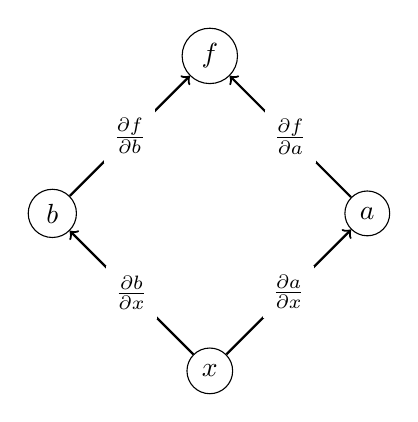
\begin{tikzpicture}
	\node[draw, circle] (f) at (0,2) {$f$};
	\node[draw, circle] (a) at (2,0) {$a$};
	\node[draw, circle] (b) at (-2,0) {$b$};
	\node[draw, circle] (x) at (0,-2) {$x$};
	
	\draw[->,thick] (x.north west) -- (b.south east) node[midway,fill=white]{$\frac{\partial b}{\partial x}$};
	\draw[->,thick] (x.north east) -- (a.south west) node[midway,fill=white]{$\frac{\partial a}{\partial x}$};
	\draw[->,thick] (a.north west) -- (f.south east) node[midway,fill=white]{$\frac{\partial f}{\partial a}$};
	\draw[->,thick] (b.north east) -- (f.south west) node[midway,fill=white]{$\frac{\partial f}{\partial b}$};
\end{tikzpicture}
	\columnbreak
	\centering
	\begin{center}
\begin{tabular}{|c|c|c|c|c|}
	\hline
	\bf Node:\phantom{\bigg|} &$x$&$a$&$b$&$f$\\
	\hline
	Value: &&&&\\
	Accumulator: &&&&\\
	\hline
	\hline
	\bf Edge:\phantom{\bigg|} &$\frac{\partial a}{\partial x}$&$\frac{\partial b}{\partial x}$&$\frac{\partial f}{\partial a}$&$\frac{\partial f}{\partial b}$\\
	\hline
	Value: &&&&\\
	\hline
\end{tabular}
	\end{center}
\end{multicols}

The first pass is forward and we calculate the values of the nodes and edges.
This is straight forward, for example, since we have $x=0.5$ and $a(x)=x^2$ the desired values are $a=0.25$ and $\frac{\partial a}{\partial x} = 1.0$
\begin{multicols}{2}
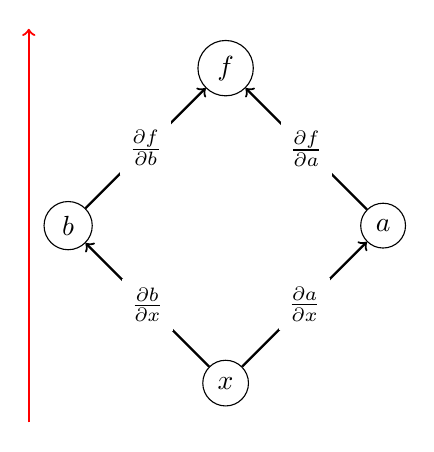
\begin{tikzpicture}
	\node[draw, circle] (f) at (0,2) {$f$};
	\node[draw, circle] (a) at (2,0) {$a$};
	\node[draw, circle] (b) at (-2,0) {$b$};
	\node[draw, circle] (x) at (0,-2) {$x$};
	
	\draw[->,thick] (x.north west) -- (b.south east) node[midway,fill=white]{$\frac{\partial b}{\partial x}$};
	\draw[->,thick] (x.north east) -- (a.south west) node[midway,fill=white]{$\frac{\partial a}{\partial x}$};
	\draw[->,thick] (a.north west) -- (f.south east) node[midway,fill=white]{$\frac{\partial f}{\partial a}$};
	\draw[->,thick] (b.north east) -- (f.south west) node[midway,fill=white]{$\frac{\partial f}{\partial b}$};
	\draw[->,red,thick] (-2.5,-2.5)--(-2.5,2.5);
\end{tikzpicture}
	\columnbreak
	\centering
	\begin{center}
\begin{tabular}{|c|c|c|c|c|}
	\hline
	\bf Node:\phantom{\bigg|} &$x$&$a$&$b$&$f$\\
	\hline
	Value: &0.5&0.25&0.125&0.25\\
	Accumulator: &&&&\\
	\hline
	\hline
	\bf Edge:\phantom{\bigg|} &$\frac{\partial a}{\partial x}$&$\frac{\partial b}{\partial x}$&$\frac{\partial f}{\partial a}$&$\frac{\partial f}{\partial b}$\\
	\hline
	Value: &1.0&0.75&0.5&1.0\\
	\hline
\end{tabular}
	\end{center}
\end{multicols}

The second pass is backwards where we set the accumulator of the output $f$ to $1$ and then recursively add the product of downstream element accumulators by edge weight to their upstream elements accumulators.

We will break this into two parts,
first part are the upstreams of the $f$ node.
The $a$ accumulator is $0.5\times1.0$ and $b$'s is $1.0\times1.0$:
\begin{multicols}{2}
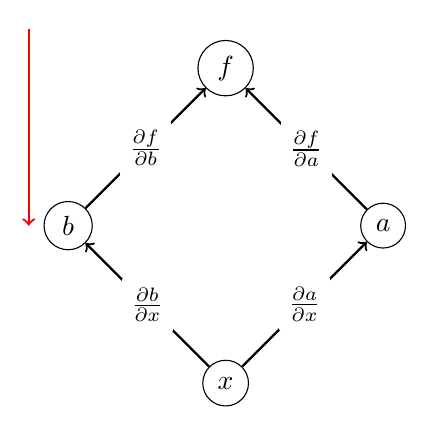
\begin{tikzpicture}
	\node[draw, circle] (f) at (0,2) {$f$};
	\node[draw, circle] (a) at (2,0) {$a$};
	\node[draw, circle] (b) at (-2,0) {$b$};
	\node[draw, circle] (x) at (0,-2) {$x$};
	
	\draw[->,thick] (x.north west) -- (b.south east) node[midway,fill=white]{$\frac{\partial b}{\partial x}$};
	\draw[->,thick] (x.north east) -- (a.south west) node[midway,fill=white]{$\frac{\partial a}{\partial x}$};
	\draw[->,thick] (a.north west) -- (f.south east) node[midway,fill=white]{$\frac{\partial f}{\partial a}$};
	\draw[->,thick] (b.north east) -- (f.south west) node[midway,fill=white]{$\frac{\partial f}{\partial b}$};
	\draw[->,red,thick] (-2.5,2.5)--(-2.5,0);
\end{tikzpicture}
	\columnbreak
	\centering
	\begin{center}
\begin{tabular}{|c|c|c|c|c|}
	\hline
	\bf Node:\phantom{\bigg|} &$x$&$a$&$b$&$f$\\
	\hline
	Value: &0.5&0.25&0.125&0.25\\
	Accumulator: &&0.5&1.0&1.0\\
	\hline
	\hline
	\bf Edge:\phantom{\bigg|} &$\frac{\partial a}{\partial x}$&$\frac{\partial b}{\partial x}$&$\frac{\partial f}{\partial a}$&$\frac{\partial f}{\partial b}$\\
	\hline
	Value: &1.0&0.75&0.5&1.0\\
	\hline
\end{tabular}
	\end{center}
\end{multicols}

And then we add continue to add the product of accumulator by edge weight to upstream nodes.
The only upstream node left is $x$ and in hence set to $0.5\times1.0+1.0\times0.75$:
\begin{multicols}{2}
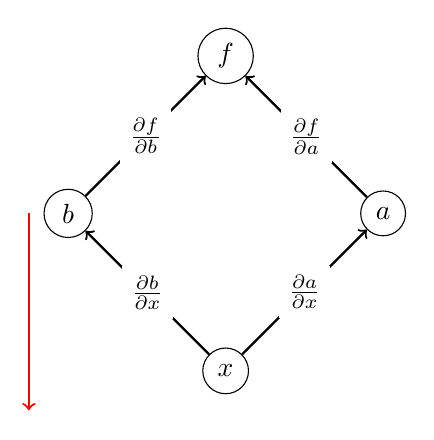
\begin{tikzpicture}
	\node[draw, circle] (f) at (0,2) {$f$};
	\node[draw, circle] (a) at (2,0) {$a$};
	\node[draw, circle] (b) at (-2,0) {$b$};
	\node[draw, circle] (x) at (0,-2) {$x$};
	
	\draw[->,thick] (x.north west) -- (b.south east) node[midway,fill=white]{$\frac{\partial b}{\partial x}$};
	\draw[->,thick] (x.north east) -- (a.south west) node[midway,fill=white]{$\frac{\partial a}{\partial x}$};
	\draw[->,thick] (a.north west) -- (f.south east) node[midway,fill=white]{$\frac{\partial f}{\partial a}$};
	\draw[->,thick] (b.north east) -- (f.south west) node[midway,fill=white]{$\frac{\partial f}{\partial b}$};
	\draw[->,red,thick] (-2.5,0)--(-2.5,-2.5);
\end{tikzpicture}
	\columnbreak
	\centering
	\begin{center}
\begin{tabular}{|c|c|c|c|c|}
	\hline
	\bf Node:\phantom{\bigg|} &$x$&$a$&$b$&$f$\\
	\hline
	Value: &0.5&0.25&0.125&0.25\\
	Accumulator: &1.25&0.5&1.0&1.0\\
	\hline
	\hline
	\bf Edge:\phantom{\bigg|} &$\frac{\partial a}{\partial x}$&$\frac{\partial b}{\partial x}$&$\frac{\partial f}{\partial a}$&$\frac{\partial f}{\partial b}$\\
	\hline
	Value: &1.0&0.75&0.5&1.0\\
	\hline
\end{tabular}
	\end{center}
\end{multicols}

The algorithm has completed and in the accumulator of each node is the partial derivative of $f$ by that node.
For example $\frac{\partial f}{\partial x} = 1.25,\,\frac{\partial f}{\partial a} = 0.5,\,\frac{\partial f}{\partial b} = 1.0,$ and $\frac{\partial f}{\partial f} = 1.0$.

\subsection{Adjoint Formula}
To see why the algorithm works we need a new math result.
While it is very similar to the partial chain rule it is in the other direction.
\\

If $x$ is upstream of $f$ and $a_n$ are immediately downstream of $x$ then we can write the partial $\frac{\partial f}{\partial x}$ as:
\[\frac{\partial f}{\partial x} = \sum_n\frac{\partial f}{\partial a_n}\frac{\partial a_n}{\partial x}\]

Informally this works because you can combine nodes together.
In our previous example we can combine $a,\,b,$ and $f$ into a single $F$:
\[F(x) = f(a(x),b(x)) = \frac{1}{2}x^2+x^3\]
\begin{center}
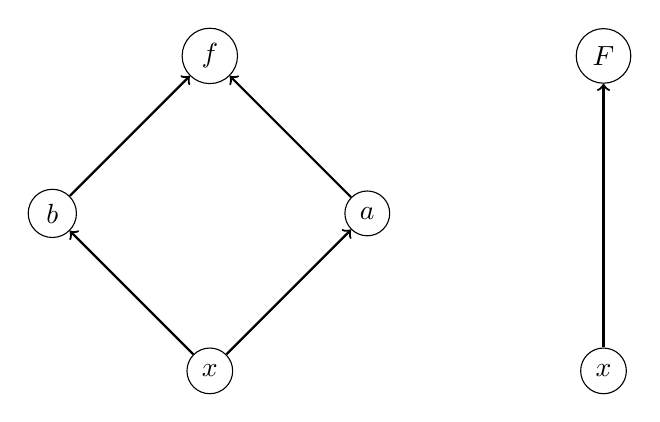
\begin{tikzpicture}
	\node[draw, circle] (f) at (0,2) {$f$};
	\node[draw, circle] (a) at (2,0) {$a$};
	\node[draw, circle] (b) at (-2,0) {$b$};
	\node[draw, circle] (x) at (0,-2) {$x$};
	
	\draw[->,thick] (x.north west) -- (b.south east);
	\draw[->,thick] (x.north east) -- (a.south west);
	\draw[->,thick] (a.north west) -- (f.south east);
	\draw[->,thick] (b.north east) -- (f.south west);

	\node[draw, circle] (X) at (5,-2) {$x$};
	\node[draw, circle] (F) at (5,2) {$F$};

	\draw[->, thick] (X.north) -- (F.south);
\end{tikzpicture}
\end{center}

To prove the adjoint relation we consider the more general case:
\begin{center}
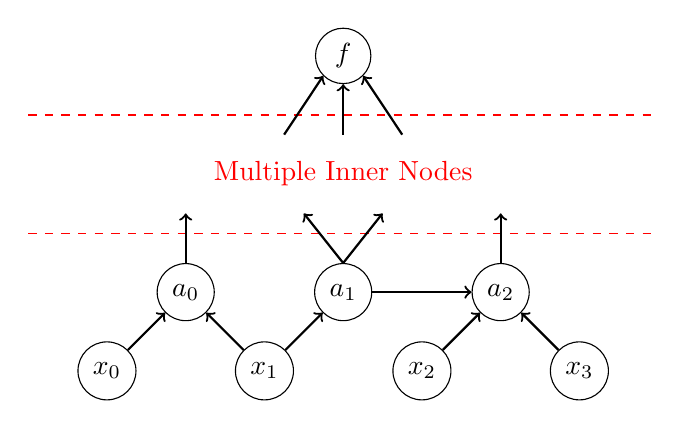
\begin{tikzpicture}
	\node[draw, circle] (x0) at (0,0) {$x_0$};
	\node[draw, circle] (x1) at (2,0) {$x_1$};
	\node[draw, circle] (x2) at (4,0) {$x_2$};
	\node[draw, circle] (x3) at (6,0) {$x_3$};
	
	\node[draw, circle] (a0) at (1,1) {$a_0$};
	\node[draw, circle] (a1) at (3,1) {$a_1$};
	\node[draw, circle] (a2) at (5,1) {$a_2$};

	\node[draw, circle] (f) at (3,4) {$f$};

	\draw[dashed, red] (-1,1.75) -- (7,1.75);
	\draw[dashed, red] (-1,3.25) -- (7,3.25);

	\draw[->,thick] (x0.north east) -- (a0.south west);
	\draw[->,thick] (x1.north west) -- (a0.south east);
	\draw[->,thick] (x1.north east) -- (a1.south west);
	\draw[->,thick] (x2.north east) -- (a2.south west);
	\draw[->,thick] (x3.north west) -- (a2.south east);

	\draw[->,thick] (a0.north) --(1,2);
	\draw[->,thick] (a1.north) --(2.5,2);
	\draw[->,thick] (a1.north) --(3.5,2);
	\draw[->,thick] (a1.east) --(a2.west);
	\draw[->,thick] (a2.north) --(5,2);

	\draw[->,thick] (2.25,3)--(f.south west);
	\draw[->,thick] (3.75,3)--(f.south east);
	\draw[->,thick] (3,3)--(f.south);

	\node[red] at (3,2.5) {Multiple Inner Nodes};
\end{tikzpicture}
\end{center}

\begin{center}
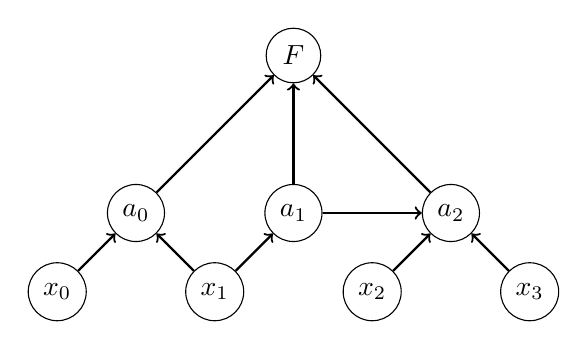
\begin{tikzpicture}
	\node[draw, circle] (x0) at (0,0) {$x_0$};
	\node[draw, circle] (x1) at (2,0) {$x_1$};
	\node[draw, circle] (x2) at (4,0) {$x_2$};
	\node[draw, circle] (x3) at (6,0) {$x_3$};
	
	\node[draw, circle] (a0) at (1,1) {$a_0$};
	\node[draw, circle] (a1) at (3,1) {$a_1$};
	\node[draw, circle] (a2) at (5,1) {$a_2$};

	\node[draw, circle] (F) at (3,3) {$F$};

	\draw[->,thick] (x0.north east) -- (a0.south west);
	\draw[->,thick] (x1.north west) -- (a0.south east);
	\draw[->,thick] (x1.north east) -- (a1.south west);
	\draw[->,thick] (x2.north east) -- (a2.south west);
	\draw[->,thick] (x3.north west) -- (a2.south east);

	\draw[->,thick] (a1.east) --(a2.west);

	\draw[->,thick] (a0.north east) -- (F.south west);
	\draw[->,thick] (a1.north) -- (F.south);
	\draw[->,thick] (a2.north west) -- (F.south east);
\end{tikzpicture}
\end{center}
\subsection{Evaluation Order}
It relates to topologies
\subsubsection{Fixed Order}
\subsubsection{Depth First}
\subsubsection{Layered}
